% Verbatim from minor_report/chapters/chapter_4_results.tex lines 1399-1707 (retired report),
% headings demoted by 1 level(s). Do not edit here; edit the source of the numbers.

\subsubsection{Question, scope, and conditions}

Trajectory error answers whether the robot knew where it was. It does not answer
whether the map it produced describes the building, nor whether a planner could
have used that map. This section evaluates the one dense map reconstructed so far
against two references of very different strength: the simulator's own collision
geometry, which is independent of the map, and the ground-truth route of the run
that built the map, which is not. The two questions are kept separate because
they fail in different ways --- a map can be geometrically faithful and still
unusable, and it can be navigable over an easy route while misrepresenting the
parts of the building that route never entered --- and because only the first
reference is independent evidence.

The evaluation is confined to the \textbf{tiny} warehouse. A large-warehouse
equivalent is \status{planned}; no database for it exists at the reporting
cutoff. Tiny-map and large-map results must not be pooled or read as repeated
trials of one condition, because the two worlds differ in extent, aisle width,
and route length. \Cref{tab:map-conditions} records the conditions.

\begin{table}[htbp]
\centering
\caption[Conditions for the dense-map evaluation.]{Conditions for the dense-map evaluation. The database and the
ground-truth route come from the \emph{same} run, which bounds what the
drivability figures can establish.}
\label{tab:map-conditions}
\small
\begin{tabularx}{\textwidth}{>{\raggedright\arraybackslash}p{0.26\textwidth}>{\raggedright\arraybackslash}X}
\toprule
Factor & Level \\
\midrule
Map under test & \repo{map/map_tiny.db}, RTAB-Map 0.23.7, created 2026-09-08 \\
World &
  \repo{aws-robomaker-small-warehouse-world/worlds/small_warehouse_static/small_warehouse_static_tinymap.world}
  (tiny geometry, despite residing in the \repo{small_warehouse_static} family
  directory) \\
Scene dynamics & static \\
Grid resolution & \SI{0.05}{\metre} \\
Geometry tolerance & \SI{0.25}{\metre} \\
Robot footprint & $0.83\times0.50$~m rectangle from
  \repo{nav2_ackermann.yaml}, not a circumscribed radius \\
World-to-map placement & $x=\SI{1.850}{\metre}$, $y=\SI{8.600}{\metre}$,
  $\theta=\SI{-89.90}{\degree}$, measured once by \repo{script/fit_map_pose.py} \\
Drivability reference, as plotted & \repo{dataset_static_tiny_repeat},
  \num{2973} poses; an independent run, no longer present in the workspace or on
  the removable drive \\
Substitute available & \repo{dataset/dataset_map_tiny},
  \repo{/ground_truth/odometry}: \num{3032} messages over \SI{60.6}{\second} of
  simulation time. This is the run that \emph{built} the map, so it is not an
  equivalent replacement \\
Evaluator & \repo{script/validate_map.py} \\
Experimental unit, $n$ & one database; $n=1$ \\
\bottomrule
\end{tabularx}
\end{table}

\subsubsection{Map placement as a validity precondition}
\label{sec:map-placement}

Both metrics depend on seating the occupancy grid in world coordinates, so
placement is a precondition rather than a display choice: a mis-seated grid
scores real structure against the wrong cells and makes a good map look bad. The
transform is a constant for a given database and is measured once, by fitting
occupied cells to the world file's wall and obstacle edges without using odometry
or ground truth. It is deliberately not taken from the live
\texttt{map~$\rightarrow$~odom} correction, which moves with front-end drift.

The measured fit is $(1.850, 8.600)\,\si{\metre}$ at \SI{-89.90}{\degree}, with a
margin of \SI{60.9}{\percent} over the best rival orientation more than
\SI{5}{\degree} away. An independent prediction --- the spawn pose of the IMU body
frame, which sits \SI{0.338}{\metre} ahead of \texttt{base\_footprint} --- gives
$(1.800, 8.662)\,\si{\metre}$. The two agree to \SI{0.080}{\metre}, inside the
grid's own \SI{0.05}{\metre} resolution. Two independent routes to the same
number is what makes this a measurement rather than a tuned parameter.

\subsubsection{Graph and database summary}

\Cref{tab:map-graph} summarizes the stored graph, read directly from the database
in read-only mode. The counts are small: \num{30} nodes over a \SI{59.3}{\second}
span, reflecting RTAB-Map's retention policy rather than the rate at which images
were offered to it.

\begin{table}[htbp]
\centering
\caption[Stored contents of \repo{map/map_tiny.db}.]{Stored contents of \repo{map/map_tiny.db}. Link rows are stored per
direction; the undirected count is the number of distinct node pairs.}
\label{tab:map-graph}
\small
\begin{tabularx}{\textwidth}{>{\raggedright\arraybackslash}p{0.30\textwidth}rr>{\raggedright\arraybackslash}X}
\toprule
Element & Rows & Undirected & Note \\
\midrule
Nodes & 30 & -- & ids 1--30, stamp span \SI{59.3}{\second} \\
Neighbour links & 56 & 28 & sequential odometry constraints \\
Global loop closures & 5 & 3 & pairs $(9,22)$, $(10,23)$, $(29,30)$ \\
Gravity links & 30 & 30 & one per node \\
Local-space links & 0 & 0 & none recorded \\
Visual words & \num{10357} & -- & vocabulary size \\
Features & \num{28374} & -- & stored keypoints \\
\bottomrule
\end{tabularx}
\end{table}

Of the three distinct closure pairs, $(9,22)$ and $(10,23)$ join nodes roughly
half a lap apart and are genuine revisits of an earlier place. The third,
$(29,30)$, joins consecutive nodes and is therefore not a revisit; it should not
be counted as evidence of place recognition.

\subsubsection{Geometry against the world file}

Geometry is scored against the rasterized collision geometry of the world file at
a \SI{0.25}{\metre} tolerance. Recall is measured against \emph{surfaces} rather
than filled interiors, because a stereo camera can only observe the outside of a
shelf; counting its interior as missed geometry would cap even a perfect map well
below \SI{100}{\percent}.

\begin{table}[htbp]
\centering
\caption{Occupied-cell geometry of \repo{map/map_tiny.db} against
\repo{small_warehouse_static_tinymap.world} at \SI{0.25}{\metre} tolerance.}
\label{tab:map-geometry}
\small
\begin{tabularx}{\textwidth}{>{\raggedright\arraybackslash}p{0.34\textwidth}r>{\raggedright\arraybackslash}X}
\toprule
Metric & Value & Population \\
\midrule
Occupied-cell precision & \SI{96.6}{\percent} & \num{11634} occupied cells \\
Recall, region the map observed & \SI{89.5}{\percent} & observed surfaces \\
Recall, whole building & \SI{67.2}{\percent} & all surfaces in the world file \\
\bottomrule
\end{tabularx}
\end{table}

The gap between \SI{89.5}{\percent} and \SI{67.2}{\percent} is route coverage, not
mapping failure: the run never entered the side aisles, so roughly a third of the
building was never observed by any sensor. The two numbers answer different
questions and neither replaces the other --- the first is a statement about
mapping quality, the second about where the robot went.

\subsubsection{Drivability against the true route}
\label{sec:map-drivability}

The robot demonstrably drove the reference route, so every pose on it was
collision-free in reality. Stamping the real footprint onto the map at each pose
therefore converts any collision into a \emph{proven} false obstacle, and any
unknown cell into a hole a planner would have to cross blind. This metric needs no
assumption about what a good map looks like.

It does, however, depend on where the route came from, and that is the weak point
of this result. The route used to produce \cref{tab:map-drivability} came from a
separate run, \repo{dataset_static_tiny_repeat}, which is no longer present in
the workspace or on the removable drive. The figures below therefore stand as a
dated independent measurement that cannot currently be re-derived.

The only surviving recording of this warehouse, \repo{dataset/dataset_map_tiny},
is not an equivalent substitute, because it is the run that built the map. Three
measurements establish this. Applying the placement of
\cref{sec:map-placement} to the stored node poses puts them a median of
\SI{0.069}{\metre} from that recording's ground-truth route; comparing each node
against the ground-truth pose carrying the \emph{same} timestamp gives a median
of \SI{0.340}{\metre} and a maximum of \SI{0.52}{\metre}; and all \num{30}
nodes fall inside the recording's sim-time interval. The second of these is the
discriminating one, since a different run over the same loop would agree in space
but not in time. The two routes are also visibly different: the lost run is a
single oval circuit, while this one is a figure-eight through the centre of the
building.

The evaluation was nevertheless repeated against this recording, and the outcome
confirms the objection rather than resolving it. Both results are reported in
\cref{tab:map-drivability}.

\begin{table}[htbp]
\centering
\caption[Drivability of \repo{map/map_tiny.db} under the true $0.83\times0.50$~m nav2 footprint, evaluated against two different routes.]{Drivability of \repo{map/map_tiny.db} under the true
$0.83\times0.50$~m nav2 footprint, evaluated against two different routes.
``Independent'' is \repo{dataset_static_tiny_repeat}, the run that did not build
the map and is no longer available. ``Build run'' is
\repo{dataset/dataset_map_tiny}, the run the map was constructed from. Geometry
is identical in both cases because it does not depend on the route.}
\label{tab:map-drivability}
\small
\setlength{\tabcolsep}{4pt}
\begin{tabularx}{\textwidth}{>{\raggedright\arraybackslash}p{0.30\textwidth}rr>{\raggedright\arraybackslash}X}
\toprule
Metric & Independent & Build run & Meaning \\
\midrule
Poses scored & \num{2973} & \num{3032} & \\
Clear and mapped & \SI{99.3}{\percent} & \SI{100.0}{\percent} & footprint free
  and observed \\
False obstacle & \SI{0.7}{\percent} & \SI{0.0}{\percent} & proven error \\
Unmapped under footprint & \SI{0.0}{\percent} & \SI{0.0}{\percent} & blind cells
  on the route \\
Clearance, median & \SI{1.07}{\metre} & \SI{1.01}{\metre} & to nearest obstacle \\
Clearance, 5th percentile & \SI{0.45}{\metre} & \SI{0.46}{\metre} & inflation
  radius is \SI{0.80}{\metre} \\
\bottomrule
\end{tabularx}
\end{table}

The difference between the two columns is the independence effect, measured rather
than assumed. Against the run that built it, the map records \emph{no} false
obstacle at all: it cannot contradict the trajectory it was constructed from. The
\SI{0.7}{\percent} that the independent run exposes is precisely the part of the
map that only a route the mapper had not seen could reveal. The right-hand column
is therefore not a better result than the left; it is a weaker question, and the
\SI{0.0}{\percent} should not be quoted as a map-quality figure.

Clearance is nearly unchanged between the two, which is expected: it is a property
of where each route runs relative to mapped geometry, not of which run built the
map. Both routes spend part of their length inside nav2's inflation radius.

\begin{figure}[htbp]
  \centering
  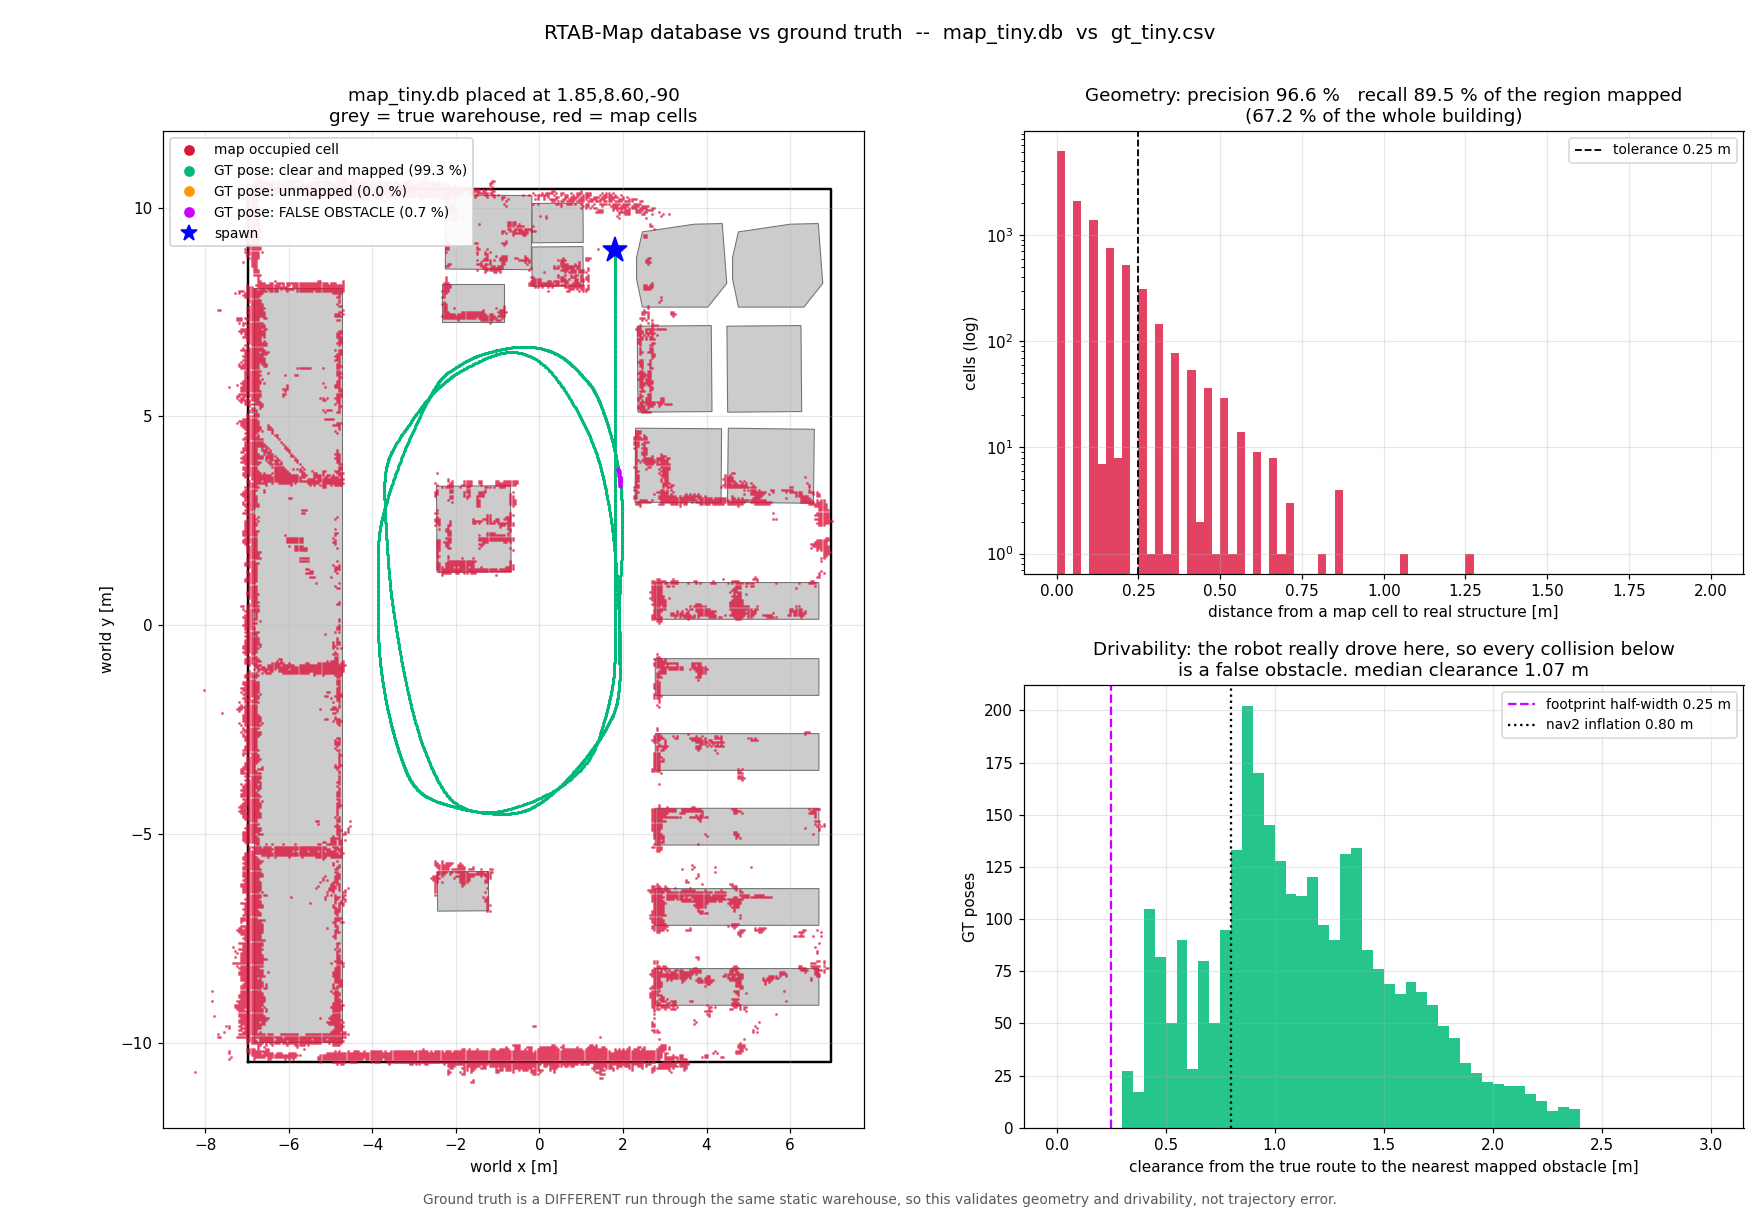
\includegraphics[width=\textwidth]{../../../output/compare/rtab_map_vs_gt.png}
  \caption[Dense-map evaluation of \repo{map/map_tiny.db}.]{Dense-map evaluation of \repo{map/map_tiny.db}. Left: occupied cells
  (red) over the world file's true collision geometry (grey), with the
  ground-truth route coloured by drivability and the spawn marked. Top right:
  distance from each occupied cell to real structure, with the
  \SI{0.25}{\metre} tolerance marked; the bulk falls well inside tolerance with a
  thin tail to about \SI{1.25}{\metre}. Bottom right: clearance from the true
  route to the nearest mapped obstacle, against the footprint half-width and the
  nav2 inflation radius. The ground truth was a different run through the same
  static warehouse, so this validates geometry and drivability, not trajectory
  error; that run is no longer available
  (\cref{sec:map-drivability}).}
  \label{fig:map-vs-gt}
\end{figure}

\begin{figure}[htbp]
  \centering
  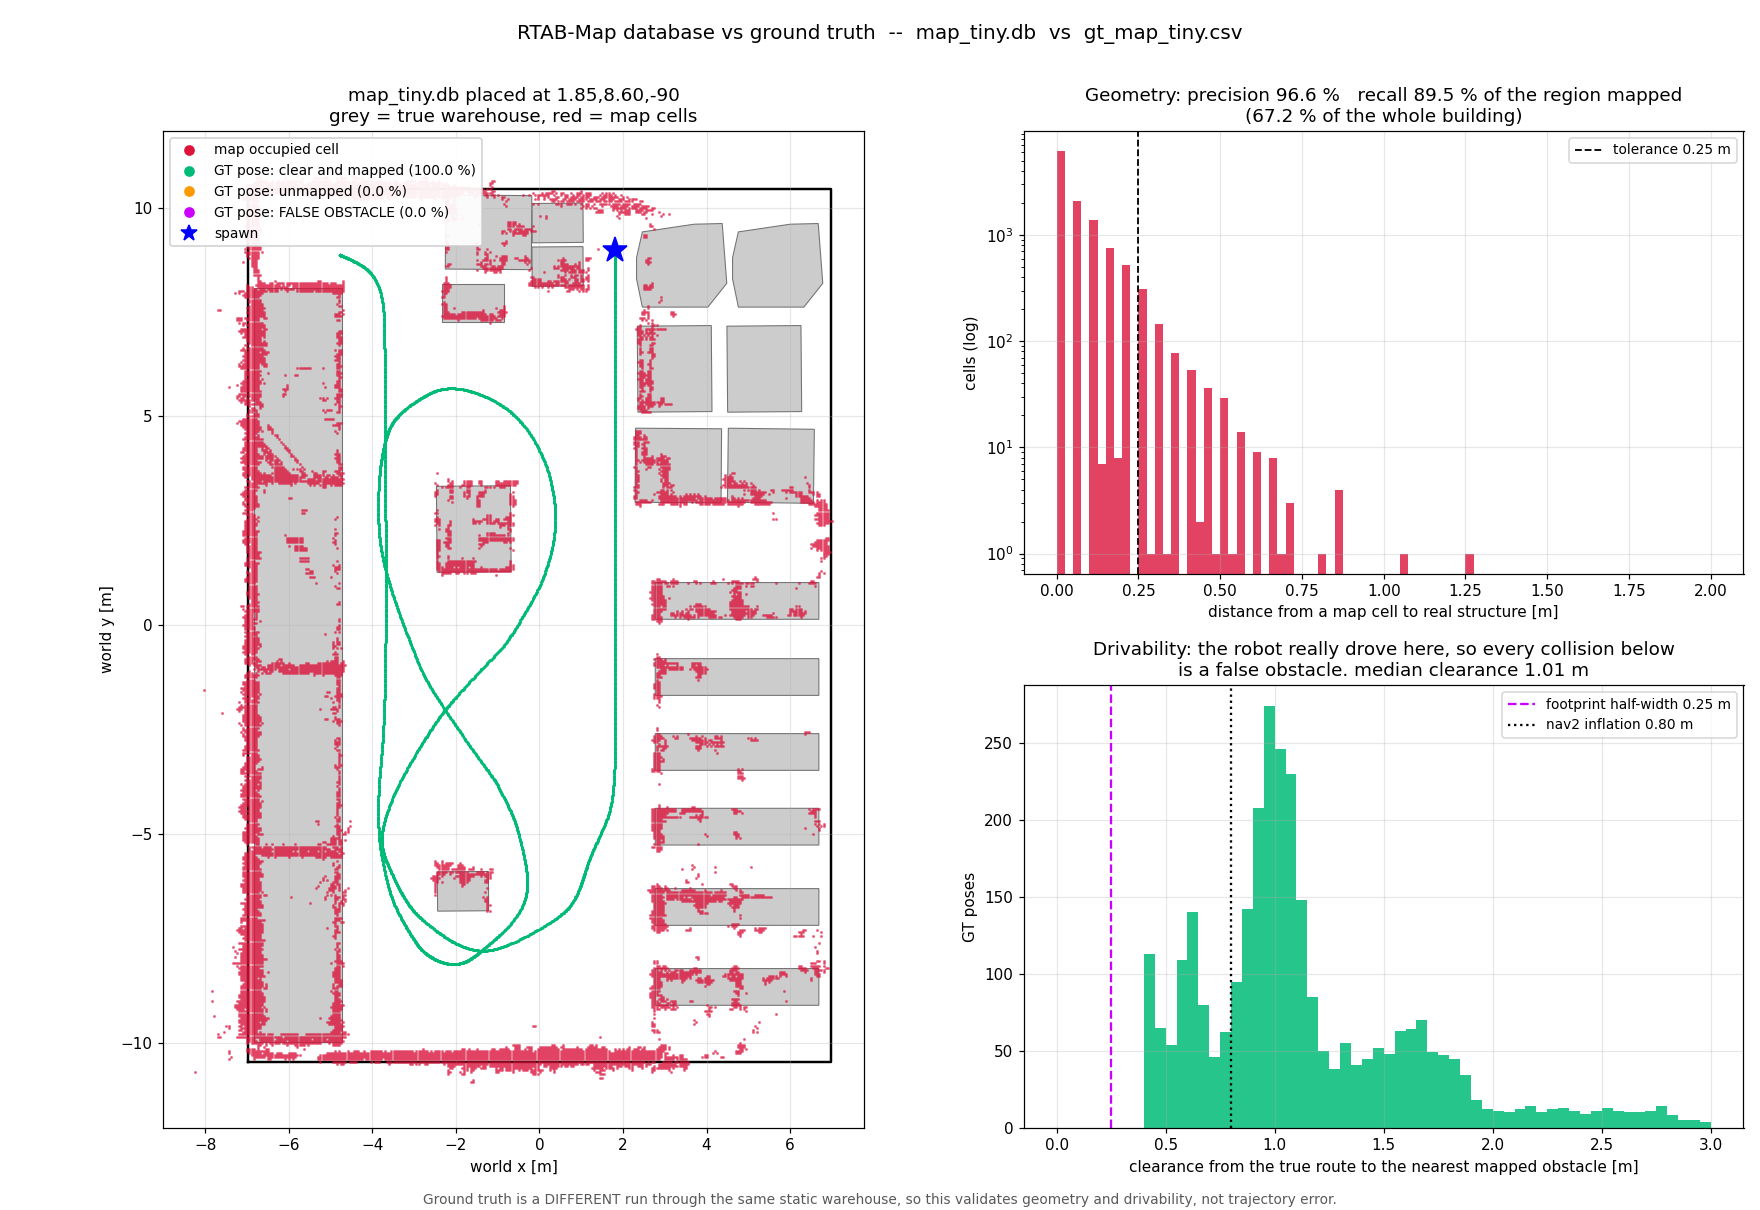
\includegraphics[width=\textwidth]{../../../output/compare/rtab_map_vs_gt_selfcheck.png}
  \caption[The same database scored against the run that built it, \repo{dataset/dataset_map_tiny}.]{The same database scored against the run that built it,
  \repo{dataset/dataset_map_tiny}. The route is a figure-eight rather than the
  oval of \cref{fig:map-vs-gt}, and no pose on it collides with the map: the
  false-obstacle rate falls from \SI{0.7}{\percent} to \SI{0.0}{\percent}. The
  geometry panels are identical to \cref{fig:map-vs-gt} because geometry does not
  depend on the route. The footer claiming a different run is emitted
  unconditionally by the evaluator and is incorrect for this figure.}
  \label{fig:map-vs-gt-selfcheck}
\end{figure}

\subsubsection{Interpretation and limitations}

Within its stated scope the tiny map is geometrically faithful and navigable:
\SI{96.6}{\percent} of what it marks as occupied is real, it recovers
\SI{89.5}{\percent} of the surfaces it actually observed, and it contains no blind
cells and only \SI{0.7}{\percent} proven false obstacles along a route the robot
really drove. The geometry half of that is independent evidence and is the
strongest map result the project currently holds; the drivability half is a
self-consistency check and is weaker than it looks. Both are a direct improvement
on earlier assessments that judged the same database unnavigable --- those were measured with the grid mis-seated, so the comparison
was against the wrong cells. That correction is a methodological finding in its
own right and is why \cref{sec:map-quality} reports placement before any metric.

Four limitations bound what these numbers support.

\begin{itemize}
  \item \textbf{The drivability reference cannot be re-read.} The run that
    provided it is lost, and the only surviving recording of this warehouse is the
    one that built the map, which would answer a weaker question. Re-establishing
    this result needs a fresh independent recording --- a second run, not a second
    map.
  \item \textbf{The route is easy.} It is one large loop down the wide central
    aisle and never squeezes into a side aisle. The \SI{0.7}{\percent} false-obstacle
    figure is therefore a floor, not a worst case. A route through the narrow
    aisles is the test that would actually stress this map, and it has not been
    run.
  \item \textbf{Clearance couples to planner cost.} The 5th-percentile clearance
    of \SI{0.45}{\metre} sits below nav2's \SI{0.80}{\metre} inflation radius, and
    a visible share of the true route lies inside it. Nothing is blocked, but a
    planner would charge a high cost for driving where the robot demonstrably
    drove. That coupling should be examined before any planned path is trusted.
  \item \textbf{$n=1$, and the scope is one world.} A single database on the tiny
    warehouse supports no uncertainty estimate and no claim about the large
    warehouse, where longer routes and narrower bays change both the drift
    exposure and the clearance margin.
  \item \textbf{Residual distortion is not a placement problem.} Walls appear
    doubled and thickened and shelf rows bowed in the overlay. No rigid transform
    removes that; it is internal map distortion and is the property that would
    limit navigation, independently of how well the grid is seated.
\end{itemize}

\begin{queried}[Queried: reproducibility of the drivability half]
The geometry result is fully reproducible: both \repo{map/map_tiny.db} and the
world file are present. The drivability result is not. Its reference run,
\repo{dataset_static_tiny_repeat}, is absent from \repo{dataset/} and from the
removable drive, and the only surviving recording of this warehouse is the one
that built the map, which would answer a weaker question
(\cref{sec:map-drivability}). The database additionally stores an empty parameter
set, so the configuration that produced it is not recoverable from the file, and
the RTAB-Map engineering record's claim that the node stamps match no dataset is
contradicted by the pose agreement reported above. The drivability figures should
therefore be read as a dated measurement rather than a standing result, and should
not be carried into the major report until an independent route has been recorded
and retained.
\end{queried}

\subsubsection{Planned extension to the large warehouse}

The same evaluation is \status{planned} for the large warehouse and is not
started: no large-map database exists at the cutoff. Three things must be settled
before those numbers would mean anything. The world-to-map placement must be
measured for the new database rather than assumed, since the tiny-map constant
$(1.850, 8.600, \SI{-89.90}{\degree})$ is specific to that database and world. A
ground-truth route must be recorded from a run \emph{other} than the one that
builds the map, which the tiny-map case did not do and which is what would turn
drivability into independent evidence. Finally, the route should deliberately
include narrow bays, so that the false-obstacle rate is exercised rather than
merely reported. Until then,
no map-quality claim extends beyond the tiny warehouse.
